\documentclass[12pt]{article}

\usepackage[english]{babel}
\usepackage[utf8x]{inputenc}
\usepackage{pdfpages}
\usepackage{lastpage} % Required to determine the last page for the footer
\usepackage{extramarks} % Required for headers and footers
\usepackage{graphicx} % Required to insert images
\usepackage{listings} % Required for insertion of code
\usepackage{courier} % Required for the courier font
\usepackage{placeins} % Required to specify float barriers
\usepackage{caption} % Required for table captions

% Margins
\topmargin=-0.45in
\evensidemargin=0in
\oddsidemargin=0in
\textwidth=6.5in
\textheight=9.0in
\headsep=0.25in

\linespread{1.1} % Line spacing

\newcommand{\Title}{CSIR - Mobile Augmented Reality Number Plate Recognition} % Project Name
\newcommand{\Class}{Requirements\ Specification} % Doc Title
\makeatletter
\renewcommand{\section}{\@startsection
   {section}%                         name
   {1}%                               level
   {0mm}%                             indent
   {-1.5\baselineskip}%               space above header
   {0.5\baselineskip}%                space under header
   {\sffamily\bfseries\upshape\normalsize}}% style
\renewcommand{\subsection}{\@startsection
   {subsection}%                      name
   {2}%                               level
   {4mm}%                             indent
   {-0.75\baselineskip}%              space above header
   {0.25\baselineskip}%               space under header
   {\rmfamily\normalfont\scshape\normalsize}}% style
\renewcommand{\subsubsection}{\@startsection
   {subsubsection}%                    name
   {3}%                               level
   {0mm}%                             indent
   {-0.75\baselineskip}%              space above header
   {0.25\baselineskip}%               space under header
   {\rmfamily\normalfont\slshape\normalsize}}% style
\makeatother


\begin{document}

        \vspace{4em}
        
        \begin{center}%
        
          \LARGE \bf \Title \\[4em]
          \LARGE {\bf Architecture Specification Proposal}\\[1em]
          \LARGE {\bf Team Members:}\\[2em]
          \large
          
             Mbulungo Musetsho                          (10176382)  \\[1em]
             Ndivhuwo Nthambeleni 						(10001183)	\\[1em]
             Joas Mogale 								(10354167)	\\[1em]
                %Enter your details below just as the one above
            
        \end{center}%
        

        \newpage
        \tableofcontents    
                \newpage
                \section{Introduction}
                		This document contains a detailed specification how the augmented reality project is going to be carried out by the Gruners group. It will specify both functional and non-functional requirements and the architectural design for the application and quality requirements. All these will be coupled with use cases for a particular system functionality and the testing thereof. This document will use an agile methodology in a sense that it will be updated as per functionality requirement from the client. 
               	%input
                \section{Vision and Scope}
                		\subsection{Vision}
                				The vision of the project is to develop a mobile application for smart phones that will enable the phone to detect vehicle number plates using a camera view and then overlaying on the display the information of the scanned vehicle. This application will then be used by mobile units to track vehicle statuses. 
                		\subsection{Scope}
                			
                				The envisioned system is a mobile application, with a web front-end, which will allow the permittted users to do the following:
                			    		\begin{itemize}
                								\item scan through number plates with the android phone
                				                \item receive the resulting information in a user-friendly display.
                				                \item make all relavent CRUD operations, using a user-friendly web interface..
                				                
                			            \end{itemize}
                		
                \section{Architectural Requirements Specification}
                		\subsection{Access Channels }
                				The envisioned system must be accessible by human users via the Android application and Web browsers.
                			
                		\subsection{Quality Requirements}
                		
                				\subsubsection{Performance}
		   			                  	The system must offer fast performance in detection of vehicle number plates as well as retrievals from the database.
		   			                  	
                			    \subsubsection{Accuracy}
                			    		Number plate detections must be at accurate. Detections made on non-stationary vehicles must be possible.
                			    		             	
                				\subsubsection{Auditability}
		   			                   	The system must maintain audits for all vital operations. These audit logs can then be provided upon request. 
		   			            		%The feature to store a scanned vehicle whose info is not yet in the DB
		   			            		
                				\subsubsection{Scalability}
	   			                   		The system must allow multiple users to make use of the application without interruptions. This holds for both the Android application and the web application.
		       			                  	
               					\subsubsection{Maintainability}
					                  	All layers of the system must be developer-friendly. - That is, the design and development of the system must allow smooth maintenance of all the system's counterparts.
       						    
       						    \subsubsection{Usability}
			    	                  	The system must allow all users to be able to interact with it without any major difficulties.
       						    	                  	
                
                		\subsection{Architecture Constraints}
                				
                				\begin{itemize}
                						\item The mobile application has to run on the Android OS with the target being Android 4.4 but allowing for compatibility with older versions up to Android 4.0.3. 
                						\item The MVC (Model View Controller) architecture pattern is to be used throughout the project.
                				\end{itemize}
               
                \section{Software Architecture Specification}
                
               		 \subsection{Architecture Requirements}
               		   
                			\subsubsection{Quality Requirements}
                					\begin{itemize}
                							\item Performance
	                								\begin{itemize}
						   			                  		\item Number plate detection must take less than 5 seconds.
						   			                  		\item Retrieval of information from the database must take no longer than 1 second.
						   			                \end{itemize}
                								
                							\item Accuracy
			              							Number plate detections must be at least 99\% accurate. Detections made on non-stationary vehicles must be possible for vehicles at most 20 metres away from the scanning device.
               								
                							\item Auditability
		               								\begin{itemize}
		               									\item The system will make audits of all operations that alter the database. .
		               									\item The system will also maintain a history of all number plate scans successfully done.
		               								\end{itemize}
		               								
		               								
                							\item Scalability
                									\begin{itemize}
					       				                  	\item The system must be able to scan all types of Southern African number plates.
					       				                  	\item The system must be able to operate effectively and efficiently under a load of 100 concurrent android application users or 100 concurrent web interface users.
					       			                \end{itemize}
		               								
                							\item Maintainability
                									To implement maintainability, the system will make use of a layered architecture that separates certain counterparts such that maintaining a subsystem does not, in any means, affect any other subsystem.
		              								
                							\item Usability
                									An average user must be able to use the system without any further training or extensive manual consultation required. This will be achieved by the use of design principles to enhance user experience.
		               								
                							
                					\end{itemize} 
                			 
                			\subsubsection{Integration and Access Channel Requirements}
                					These are the dirrent channels through which the system can be accessed by all related users.
	                				The system will be accessible by human users through the following channels:
	                				
			                    	\begin{enumerate}
					                    	\item From the web browser throuch a user-friendly web interface. This implies that the system must be accessible from all widely used web browsers (including the most recent versions of Mozilla Firefox, Google Chrome, Apple Safari and Microsoft Internet Explorer).
					                    	\item From mobile android devices using the Android application.
			                    	\end{enumerate}  
			                    	  
                			\subsubsection{Architecture Constraints}
                					The following architecture constraints will be followed mainly for maintainability reasons:
                					\begin{enumerate}
                							\item All system counterparts must be developed and attached to a JAVA RESTful Web Service.
                							\item The business logic layer must provide an API for access to the SQL Database.
                							\item The system will make use of the MySQL database.
                							\item The mobile client must run on an Android application.
                							\item The system functionality will be hidden in a RESTful web services such that it is not exposed to any presentation layer counterpart.
                					\end{enumerate}
                				
                			  
                	\subsection{Architectural patterns or Styles}
                			For the sake of good high-level responsibility separation and allowance for reuse of lower level layer components across components in higher level layers, a layered architecture will be used for this system.
                			The layered architecture for the system contains the following layers:
                			\begin{itemize}
		                			\item Client Layer
		                			\item Access Layer
		                			\item Business Processes Layer
		                			\item Domain Objects Layer
		                			\item Backend Layer
                			\end{itemize} 
                			
                			
                			\begin{figure}[h]
                                   \centering
                                   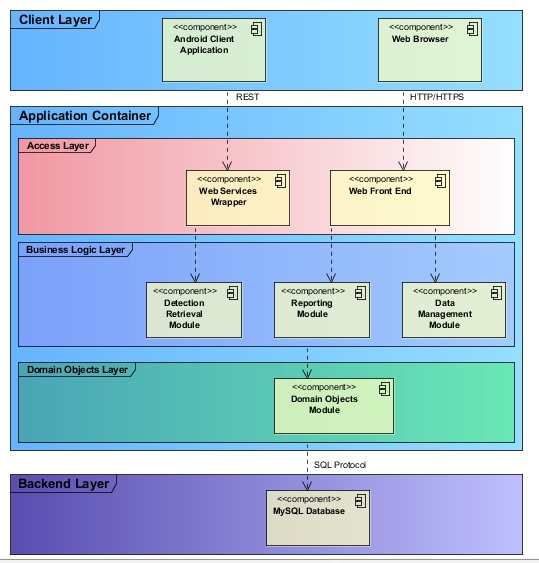
\includegraphics[width=3.59in, height=3.75in]{Pictures/SystemArchitectureLayers.jpg}
                                   \caption{System Layered Architecture}
        					\end{figure}
        					\FloatBarrier
                			
                			
                			The responsibility allocation across the layers is as follows:
                			\begin{enumerate}
                					\item Provide access to humans: Client Layer
                					\item Provide access to system functionality to human access layer and other systems: Access Layer
                					\item Business Logic Encapsulation: Business Processes Layer
                					\item Provide domain objects: Domain Objects Layer
                					\item Hosting Database: Backend Layer
                			\end{enumerate}
                			
                    % Commented out for later stage:\subsection{Architecture Tactics or Strategies}
                    % Commented out for later stage: \subsection{Use of Reference Architecture and Frameworks }
					\subsection{Technologies}
							Technologies that will be used throughout the system development include:
							\begin{itemize}
								\item JAVA Native Android SDK
								\item HTML 5
								\item JAVA Programming Language
								\item Qualcomm Vuforia Augmented Reallity SDK
								\item MySQL Database for JDBC
							\end{itemize}
                    
                %\section{Functional requirements and application design}
                    %\subsection{Introduction}
                   % \subsection{Required functionality}
                   % \subsection{Use case prioritization}
                   % \subsection{Use Case/Services contracts}
                   % \subsection{Process specifications}
                   % \subsection{Domain Objects}
               %\section{Glossary}
             
\end{document}


